
\begin{figure*}[ht!]
  \centering
  \begin{subfigure}[t]{\textwidth}
    \begin{subfigure}[t]{0.19\linewidth}
      \centering
      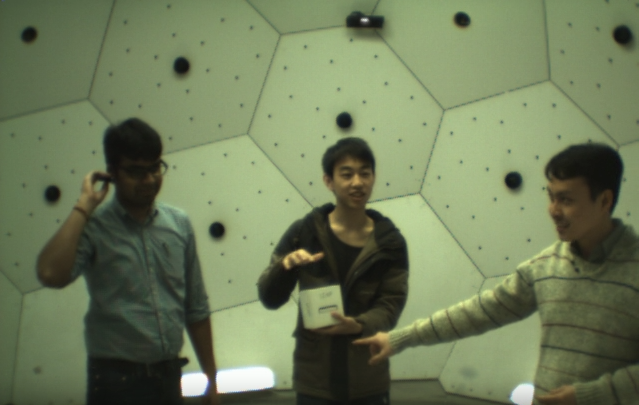
\includegraphics[width=\linewidth]{figures/examples/example1.png}
    \end{subfigure}
    \begin{subfigure}[t]{0.19\linewidth}
      \centering
      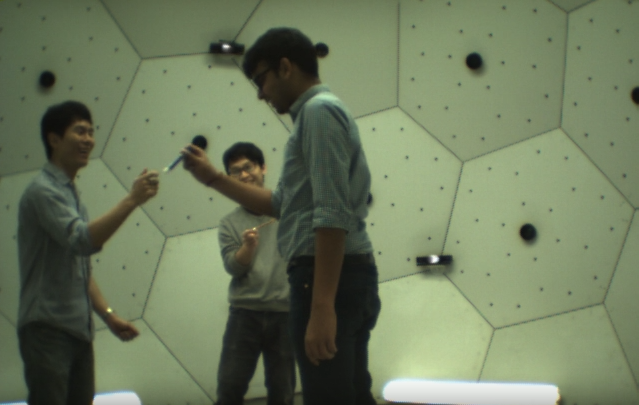
\includegraphics[width=\linewidth]{figures/examples/example2.png}
    \end{subfigure}
    \begin{subfigure}[t]{0.19\linewidth}
      \centering
      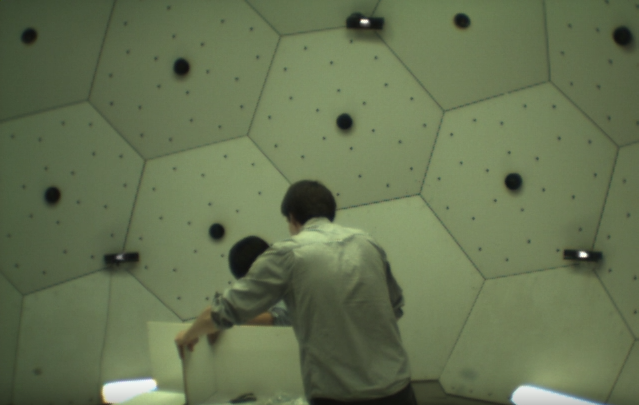
\includegraphics[width=\linewidth]{figures/examples/example3.png}
    \end{subfigure}
    \begin{subfigure}[t]{0.19\linewidth}
      \centering
      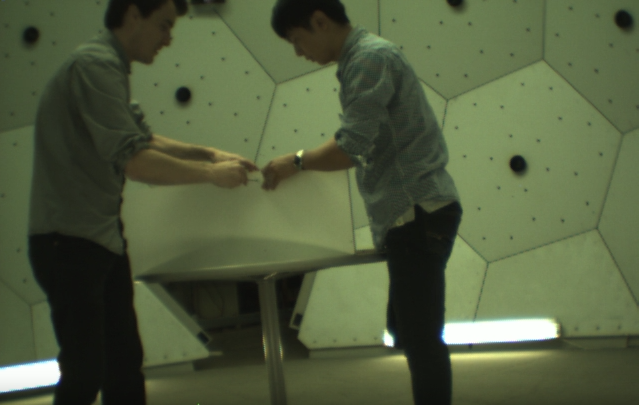
\includegraphics[width=\linewidth]{figures/examples/example4.png}
    \end{subfigure}
    \begin{subfigure}[t]{0.19\linewidth}
      \centering
      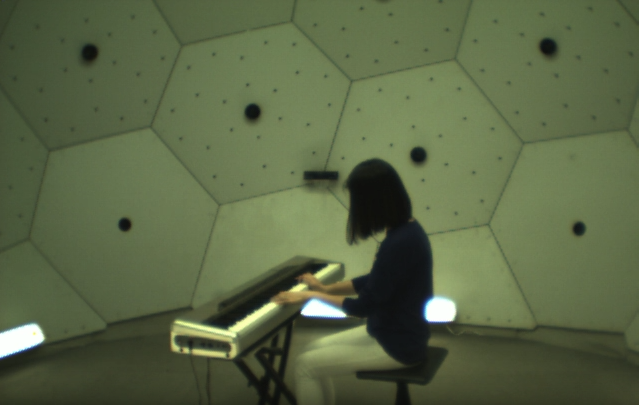
\includegraphics[width=\linewidth]{figures/examples/example5.png}
    \end{subfigure}
  \end{subfigure}
  \begin{subfigure}[t]{\textwidth}
    \begin{subfigure}[t]{0.19\linewidth}
      \centering
      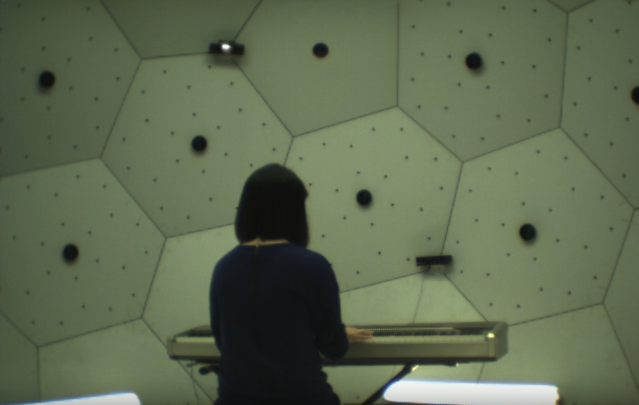
\includegraphics[width=\linewidth]{figures/examples/example6.png}
    \end{subfigure}
    \begin{subfigure}[t]{0.19\linewidth}
      \centering
      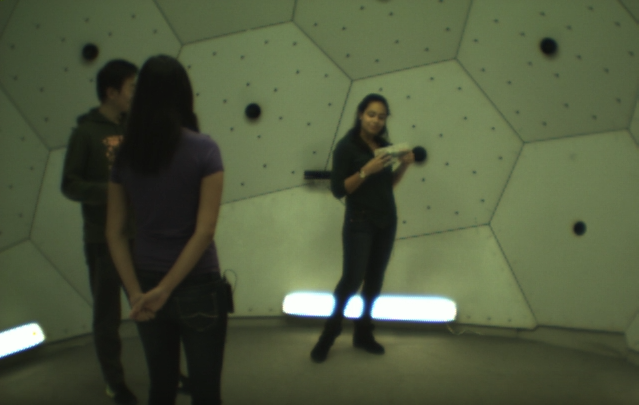
\includegraphics[width=\linewidth]{figures/examples/example7.png}
    \end{subfigure}
    \begin{subfigure}[t]{0.19\linewidth}
      \centering
      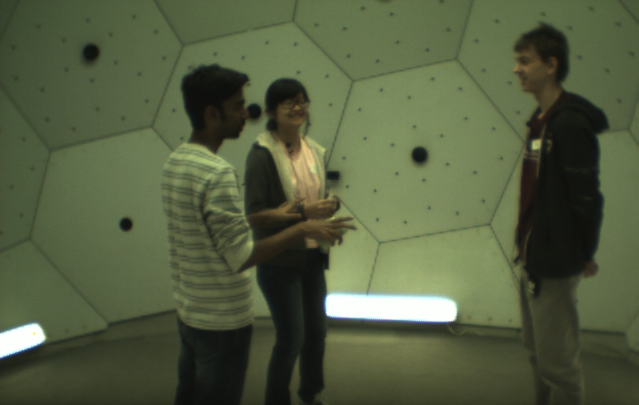
\includegraphics[width=\linewidth]{figures/examples/example8.png}
    \end{subfigure}
    \begin{subfigure}[t]{0.19\linewidth}
      \centering
      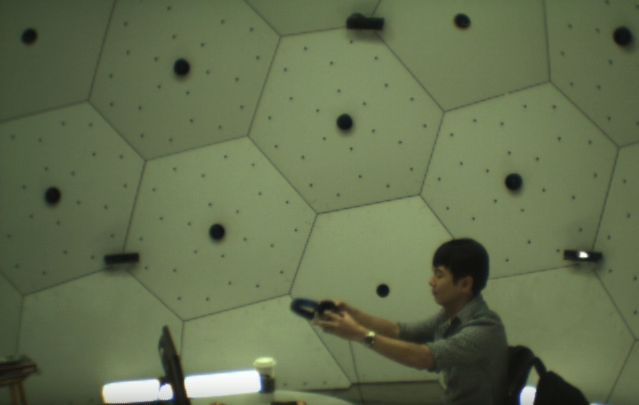
\includegraphics[width=\linewidth]{figures/examples/example9.png}
    \end{subfigure}
    \begin{subfigure}[t]{0.19\linewidth}
      \centering
      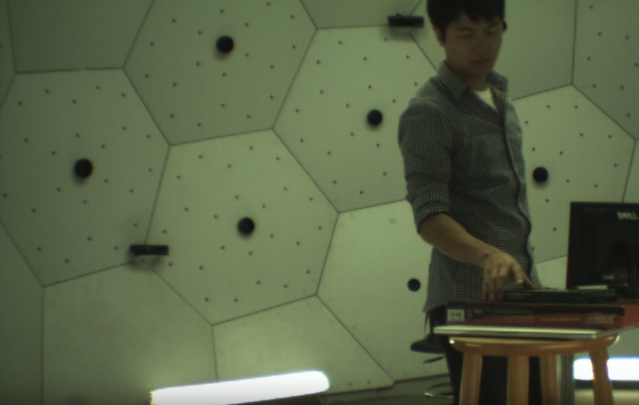
\includegraphics[width=\linewidth]{figures/examples/example10.png}
    \end{subfigure}
  \end{subfigure}
  \caption{A series of example images extracted from the video sequences of the CMU Panoptic dataset.}
  \label{fig:examples}
\end{figure*}

\section{Experimental Evaluation} \label{experiments}

This section of the report will focus on how the proposed system has been experimentally evaluated. Further it covers the dataset used for the experiments and the selected evaluation metrics.


\subsection{Dataset Description} \label{dataset-desc}

For the development and evaluation of the tracking system in this project, the CMU Panoptic Dataset \parencite{Joo_2015_ICCV,Joo_2017_TPAMI,Simon_2017_CVPR} has been used. This is a large-scale dataset that was originally recorded to facilitate research in multi-view social motion capture. \Cref{fig:examples} shows a sample of some still images extracted from the video sequences contained in this dataset.

The complete dataset includes 84 video sequences totaling approximately 11.5 hours of video captured in a specialized 5.49m diameter dome-shaped room equipped with inward facing cameras attached to the outside panels. In total, the recording hardware consists of 511 calibrated cameras, 480 VGA cameras recording at a $640 \times 480$ resolution at 25 fps and 31 HD cameras recording at a $1920 \times 1080$ resolution at 30 fps. The room also contains 10 Kinect II \parencite{kurillo2022evaluating} sensors and 5 DLP projectors. Because of the geometry of the room and the placement of cameras, no single camera is able to view the complete space. This means that while each point in the space is visible from multiple cameras, each camera only captures a partial view of the environment, introducing occlusion and field-of-view limits related challenges for the tracking task.

Crucially, the dataset also includes ground truth 3D skeletons and tracks that were generated by the CMU researchers using algorithms that leverage the entirety of the camera array \parencite{Joo_2015_ICCV}. Ground truth annotations of the dataset are provided in the COCO19 format. To align them with the outputs of the YOLO-based pose estimation networks used in this project \parencite{ultralyticsYOLO}, the ground truth data was pre-processes by converting it into the COCO17 format \parencite{lin2014microsoft}. This was achieved by discarding the two extra joint positions. The dataset also includes the calibration parameters for all available camera views, including camera extrinsics, intrinsics, and distortion parameters.

% TODO change the list of sequences that have been used for testing
Due to computational and time constraints, running the tracking system across all the sequences for the dataset was not reasonable. For this reason, a subset of the dataset was selected for use as the testing set. These sequences where also excluded from the training of the system components as explained in \cref{arch-learning}. The following eight sequences were reserved for testing: \inlinecode{160224_haggling1}, \inlinecode{160906_ian1}, \inlinecode{160906_pizza1}, \inlinecode{161029_build1}, \inlinecode{161029_sports1}, \inlinecode{170221_haggling_m3}, \inlinecode{170915_office1}, and \inlinecode{171026_pose3}. These sequences have been selected to cover a wide verity of different and challenging scenarios. Furthermore, evaluation was performed using only a subset of all camera views. A maximum of 16 VGA-type cameras were utilized per video sequence. These 16 cameras were selected based on the official dataset download script \footnote{\url{https://github.com/CMU-Perceptual-Computing-Lab/panoptic-toolbox/blob/master/scripts/getData.sh}}, which ensures they are approximately uniformly distributed around the dome to provide maximum spatial coverage with a minimal camera count.

In addition to the CMU Panoptic dataset, for some qualitative analysis and demos also the SALSA dataset \parencite{alameda2015salsa} has been used. This dataset represents a much more difficult scenario for the system, however, because it does not contain any ground truth pose annotations, it could not be used for the quantitative evaluations.

\begin{table*}[!ht]
  \centering
  \begin{tabular}{|r|r|c|c|c|c|c|c|c|}
  \hline
    Model & \# Cameras & Detection & Matching & EKF Update & EKF Prediction & Total \\ \hline
    \multirow{4}{*}{YOLO26n-pose}  & 4 & 0.0411 & 0.0131 & 0.0069 & 0.0005 & 0.0616 \\ \cline{2-7}
      & 8 & 0.0850 & 0.0236 & 0.0102 & 0.0007 & 0.1195 \\ \cline{2-7}
      & 12 & 0.1403 & 0.0280 & 0.0118 & 0.0008 & 0.1809 \\ \cline{2-7}
      & 16 & 0.1922 & 0.0355  & 0.0163 & 0.0008 & 0.2448 \\ \hline \hline
    YOLO26s-pose & 4 & 0.1137 & 0.0139 & 0.0083 & 0.0007 & 0.1365 \\ \hline
    YOLO26m-pose & 4 & 0.2866 & 0.0140 & 0.0087 & 0.0007 & 0.3100 \\ \hline
    YOLO26l-pose & 4 & 0.3408 & 0.0143 & 0.0090 & 0.0007 & 0.3648 \\ \hline
  \end{tabular}
  \caption{Average per-frame runtime of the tracking system for different camera and model configurations. Times are given in seconds.}
  \label{fig:perf}
\end{table*}

\begin{table*}[!ht]
  \centering
  \begin{tabular}{|r|r|c|c|c|c|c|}
  \hline
    Model & \# Cameras & MOTA & MOTP & MPJPE & Precision & Recall \\ \hline \hline
    \multirow{4}{*}{YOLO26n-pose} & 4 & 0.781 & 5.488 & 8.250 & 0.890 & 0.890 \\ \cline{2-7}
      & 8 & 0.924 & 3.235 & 3.341 & \textbf{0.939} & 0.994 \\ \cline{2-7}
      & 12 & \textbf{0.926} & 3.066 & 3.146 & 0.939 & 0.996 \\ \cline{2-7}
      & 16 & 0.920 & \textbf{2.749} & \textbf{2.834} & 0.934 & \textbf{0.996} \\ \hline \hline
    YOLO26s-pose & 4 & 0.785 & 5.151 & 8.616 & 0.888 & 0.899 \\ \hline
    YOLO26m-pose & 4 & 0.807 & 4.976 & 7.466 & 0.897 & 0.913 \\ \hline
    YOLO26l-pose & 4 & 0.809 & 4.792 & 7.674 & 0.898 & 0.915 \\ \hline
  \end{tabular}
  \caption{Evaluation results for the baseline configuration with different camera and model configurations. MOTA, MOTP, Precision, and Recall have been computed with an average of 15 centimeters Euclidean distance as the matching threshold. MOTP and MPJPE are given as mean per-joint Euclidean distance in centimeters. The best result in each column is highlighted in bold.}
  \label{fig:eval-results}
\end{table*}


\subsection{Evaluation Procedure} \label{eval-proc}

For this project the system has been evaluated by comparing its 3D tracking predictions frame-by-frame against the ground truth annotations in the CMU Panoptic dataset. The experiments were run across all eight selected sequences mentioned in \cref{dataset-desc}, evaluating various combinations of YOLO pose estimation models, testing \inlinecode{YOLO26n-pose}, \inlinecode{YOLO26s-pose}, \inlinecode{YOLO26m-pose}, and \inlinecode{YOLO26l-pose}, spacial view densities of 4, 8, 12, and 16, as well as testing different configurations of the system, such as with or without skeletal constraints. Note only the \inlinecode{YOLO26n-pose} model has been tested with more than 4 cameras and that the more advanced configurations of the system have also only been tested in the 4 camera setting. All evaluations were performed on AMD Ryzen AI 9 HX 370 CPU with most PyTorch \parencite{paszke2019pytorch,ansel2024pytorch} operation running on the integrated AMD Radeon 890M GPU.

For the baseline system configuration, parameters of the system were initialized heuristically rather than via exhaustive grid-search or end-to-end learning. While these rigid parameter values are functional, the system performs better when using the components that were learned from data as shown in \cref{results}.

For the baseline system, detection thresholds for the YOLO based detector we set to $\tau_{obj} = 0.5$ and $\tau_{kpt} = 0.25$, using also $N_{kpt} = 3$ as the minimum number of visible keypoints. The minimum pixel variance has been set to $\sigma_{min}^2 = 16.0$ pixels$^2$, with visibility and invisibility scale variances set to $\sigma_{vis}^2 = 0.005$ and $\sigma_{inv}^2 = 5$. The matching thresholds for both cross-view and prediction-view matching have both been set to $\theta_{mn} = \theta_{mo} = 0$. For the tracking lifecycle we configured the age for tentative track promotion to $N_{age} = 3$ and the maximum duration without detections for active tracks to $N_{inv} = 10$. Finally, the continuous physic matrices have been set as follows:
\begin{align*}
    \mathbf{F} = \begin{bmatrix} \mathbf{0}_{51 \times 51} & \mathbf{I}_{51 \times 51} \\ \mathbf{0}_{51 \times 51} & -0.2 \cdot \mathbf{I}_{51 \times 51} \end{bmatrix}, & \;
    \mathbf{Q} = \begin{bmatrix} \sigma_{p}^2 \cdot \mathbf{I}_{51 \times 51} & \mathbf{0}_{51 \times 51} \\ \mathbf{0}_{51 \times 51} & \sigma_{v}^2 \cdot \mathbf{I}_{51 \times 51} \end{bmatrix}
\end{align*}
with $\sigma_{v}^2 = (3 \frac{m}{s})^2$ and $\sigma_{p}^2 = (1 cm)^2$. This matrix models constant velocity dynamics with a damping term of $-0.2$ on velocity to stabilize motion predictions.


\subsection{Evaluation Metrics} \label{eval-metrics}

To measure tracking and reconstruction performance, this project makes use of standard metrics from the Multi-Object Tracking and 3D Pose Estimation literature \parencite{bernardin2008evaluating,ionescu2013human3}. All measures are reported in centimeters, and we use a mean joint error of 15 centimeters as the threshold for matches for all metrics except MPJPE.

\paragraph{Mean Per-Joint Position Error (MPJPE)}
MPJPE measures the average 3D Euclidean distance between predicted and ground truth keypoints across all matched frames and joints.
\begin{align*}
    \text{MPJPE} &= \frac{1}{N_{matched}} \sum_{i=1}^{N_{matched}} \left( \frac{1}{17} \sum_{k=1}^{17} \|\mathbf{p}_{k,i}^{pred} - \mathbf{p}_{k,i}^{gt}\|_2 \right)
\end{align*}
For this metric we do not apply a matching threshold, instead matching all predictions against the best matching ground truth track via Hungarian method based assignment.

\paragraph{Multi-Object Tracking Accuracy (MOTA)}
MOTA evaluates overall tracking performance by accounting for three types of errors, false positives, false negatives, and identity switches:
\begin{align*}
    \text{MOTA} &= 1.0 - \frac{\sum_{t} \text{FN}_t + \text{FP}_t + \text{IDS}_t}{\sum_{t} \text{GT}_t}
\end{align*}
where $\text{FN}_t$ is the number of false negatives, $\text{FP}_t$ the number of false positives, $\text{IDS}_t$ that of identity switches, and $\text{GT}_t$ is the number of ground truth individuals in frame $t$.

\paragraph{Multi-Object Tracking Precision (MOTP)}
MOTP measures the alignment of tracked objects by calculating the average distance error for correctly matched targets. Note that in contrast to MPJPE this metric is only computed over the true positives matched within the 15 centimeters maximum threshold.
\begin{align*}
    \text{MOTP} &= \frac{\sum_{t,d} \frac{1}{17} \sum_{k=1}^{17} \|\mathbf{p}_{t,d,k}^{pred} - \mathbf{p}_{t,d,k}^{gt}\|_2}{\sum_{t} \text{TP}_t}
\end{align*}
where $\text{TP}_t$ is the number of true positives.

\paragraph{Precision and Recall}
Finally, we also report the standard precision and recall metrics.
\begin{align*}
    \text{Precision} = \frac{\sum_t \text{TP}_t}{\sum_t \text{TP}_t + \text{FP}_t}, &\quad \text{Recall} = \frac{\sum_t \text{TP}_t}{\sum_t \text{TP}_t + \text{FN}_t}
\end{align*}
